\section{Throwing Booth}
\label{sec:booth}
The booth is constructed from Item Profiles.
The objects are thrown through in front of a constant background, therefore there is a white back wall opposite the camera.
When creating the booth design, care was taken to ensure that the size corresponds to the width of a table (750mm).
This also defined the distance between the camera and the back wall.
With the opening angle of the lens, the minimum required size of the back wall can be calculated as in equation \ref{eq:Fieldwith}. 
In the following this size is called field of view.

\begin{equation}
	f_w = 2*a*tan\left( \frac{\vartheta}{2}\right) = 690mm
	\label{eq:Fieldwith}
\end{equation}

Whereby the following applies:
\begin{itemize}
	\item $f_w$ = width of the field of view
	\item $a$ = Distance camera to back panel = 630mm
	\item $\vartheta$ = horizontal angle of view = 57.4° \cite{BaumerLense}
\end{itemize}

Assuming that the picture format is 1280x1024, the height of the field of view can also be calculated:

\begin{equation}
	f_h = f_w*\frac{1024}{1280} = 552mm
	\label{eq:Fieldhight}
\end{equation}

The objects should be passed as far away from the camera as possible to be able to take more pictures per throw.
To ensure that the objects are thrown through the field of view and far away from the camera, there is a hole in the back wall as a target.
It is located on the right side of the back wall, which is further away from the camera.
If the throwing objects are hit through the hole in the rear wall, they land in a net.

The throwing booth is drawn in the CAD tool Inventor.
The camera is mounted on the Item profile with an aluminum mounting adapter which is shown in figure \ref{fig:mounting_adapter} and protected from damage with an aluminum sheet.
The drawings of these parts can be found in the appendix \ref{app:drawings_mounting_adapter} and \ref{app:drawings_camera_protection}.

In order to detect and correct errors in thinking, the booth with all its components was designed using a 3D model.
This also includes a case in which the electronics can be stowed away.
The case is a container from Fibox with a transparent lid.
The construction drawings can be found in the appendix \ref{app:drawings_fibox_bottom}.

\begin{figure}[h]
	\centering
	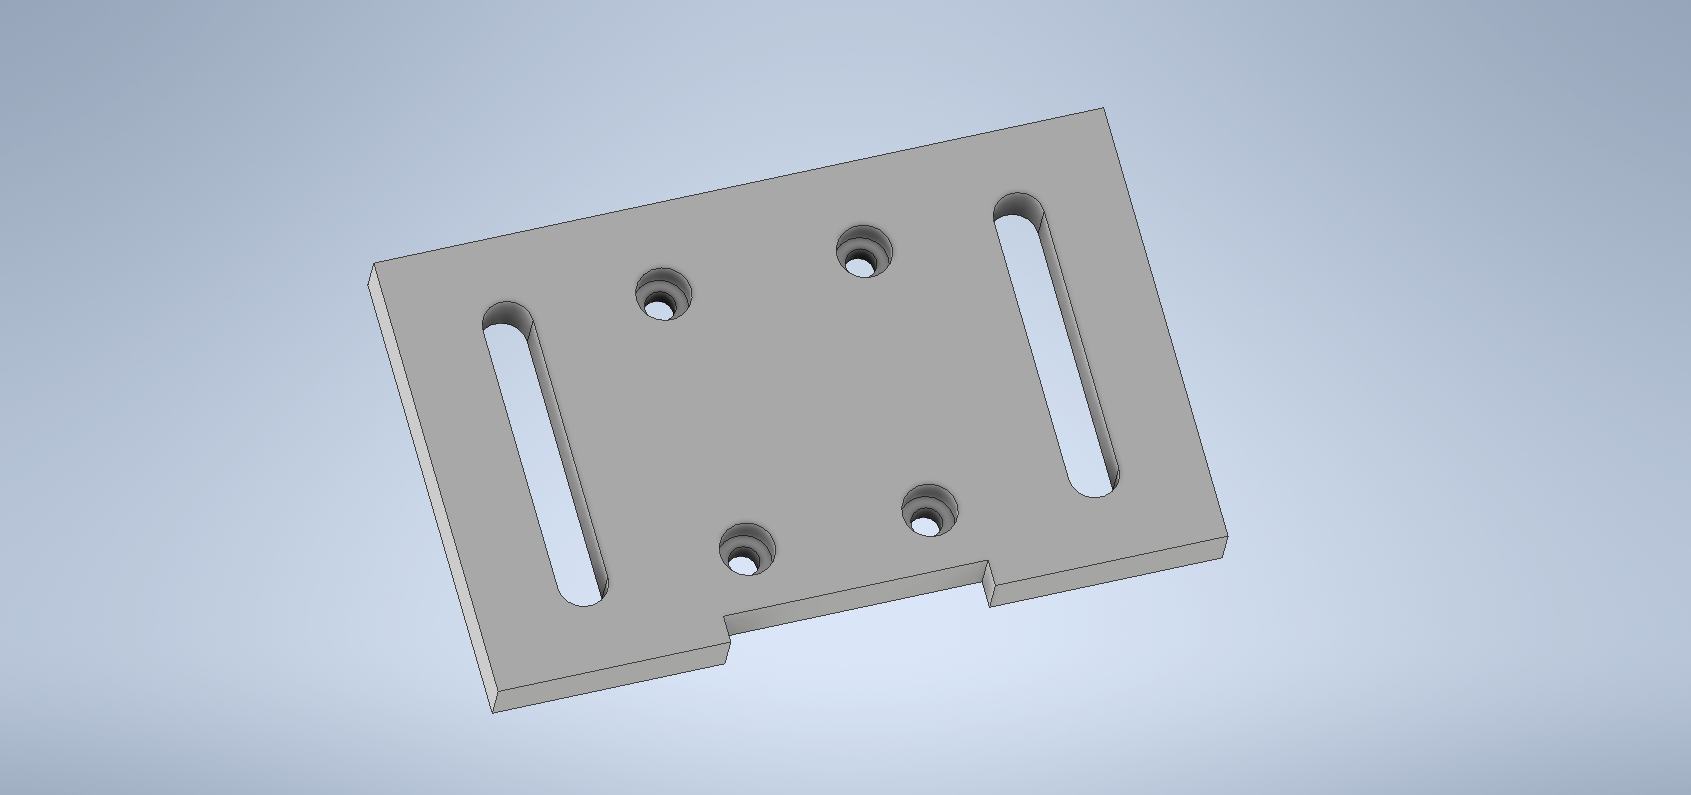
\includegraphics[scale=0.2]{graphics/mounting_adapter.png}
	\caption{Mounting Adapter}
	\label{fig:mounting_adapter}
\end{figure}


